\chapter{Complementary-Filter}
\label{chap:ComplementaryFilter}

As written in the chapter about the sensor fusion for the complementary filter a filter time needs to be chosen. This constant is used for the lowpass filter for the acceleration/magnetic sensor and for the highpass filter of the gyroscope. \\\\
The complementary filter uses the following calculation:
\begin{align}
angle=alpha*(angle+integrated\_Gyro)+(1-alpha)*Acc\_Mag\_angle
\label{equ:Comp1}
\end{align}

As an initial guess for the first try the complementary filter uses the filter constant of 0.995. The sampling period of the sensors is 800 Hz. Usage of the filter constant of 0.995 and the sampling period of 800 Hz leads to a cut off frequency of 4 Hz. 
\begin{align}
alpha&=\frac{time\_constant}{time\_constant+sample\_period}
\label{equ:Comp2}
\end{align}
\begin{align}
alpha&=0.995\\
sample\_period&=\frac{1}{800 Hz}=0.00125sec\\
\label{equ:Comp2}
\end{align}
This leads to:
\begin{align}
time\_constant = 0.2488sec\approx \frac{1}{4 Hz}
\label{equ:Comp3}
\end{align}
With this constant the following result was achieved. To make a test, first the yaw angle is changed in the range of $\pm90 \degree$, after that a roll angle is changed in the range of $\pm90 \degree$ and finally the pitch angle is changed in the range of $\pm90 \degree$.

\begin{figure}[H]
	\centering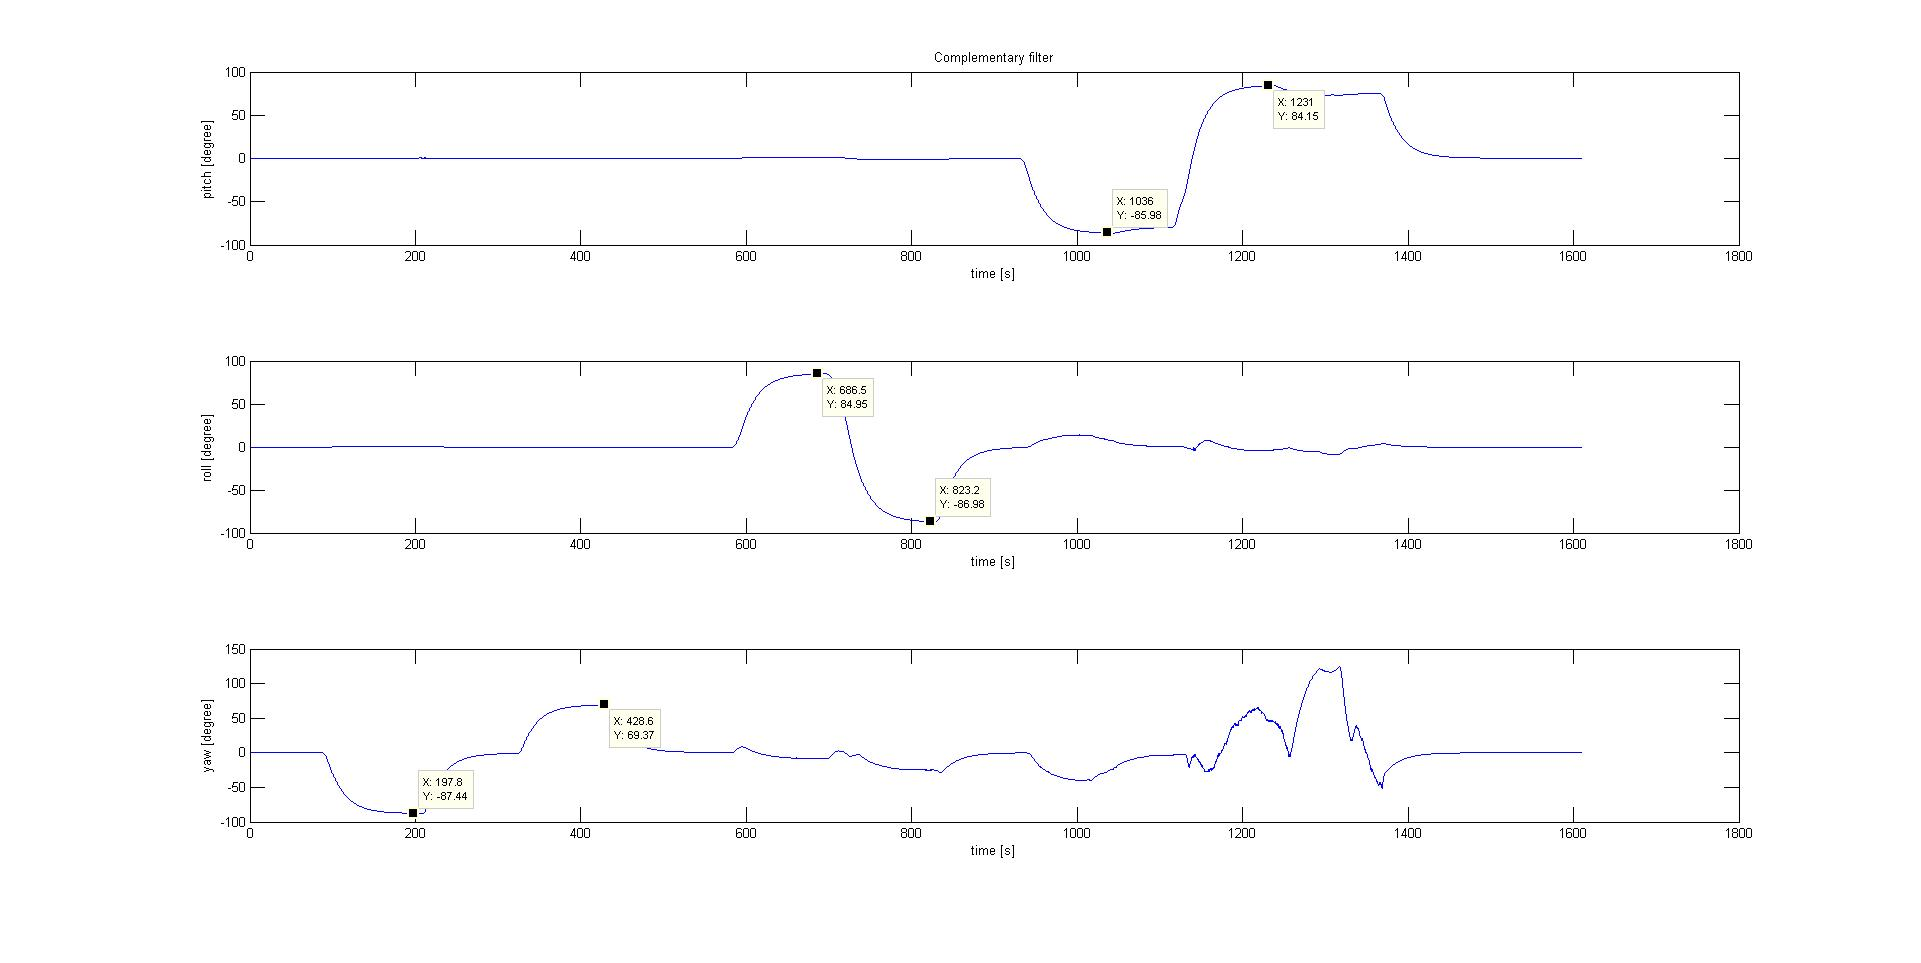
\includegraphics[width=1.0\textwidth]{fig/initial_Comp}
	\caption{First result complementary filter}
	\label{fig:initial_Comp}
\end{figure}

First what catches somebodys eye is that the filter is to slow. So the steady state value is achieved after consuming to much time. Also the yaw angle is not equally distributed over the whole 360 degree. In one direction the angle changes just around 70 degree. When changing roll the influences in yaw is just because the rotation was not straight in roll direction. Changing the pitch angle to much lead to a change in yaw. The next step is to improve the yaw angle, so that it will reach also the +90 degree. Also the yaw change during pitch will be observed and compared to the initial measurement. Also the time constant will be changed that a faster response can be seen.
\begin{figure}[H]
	\centering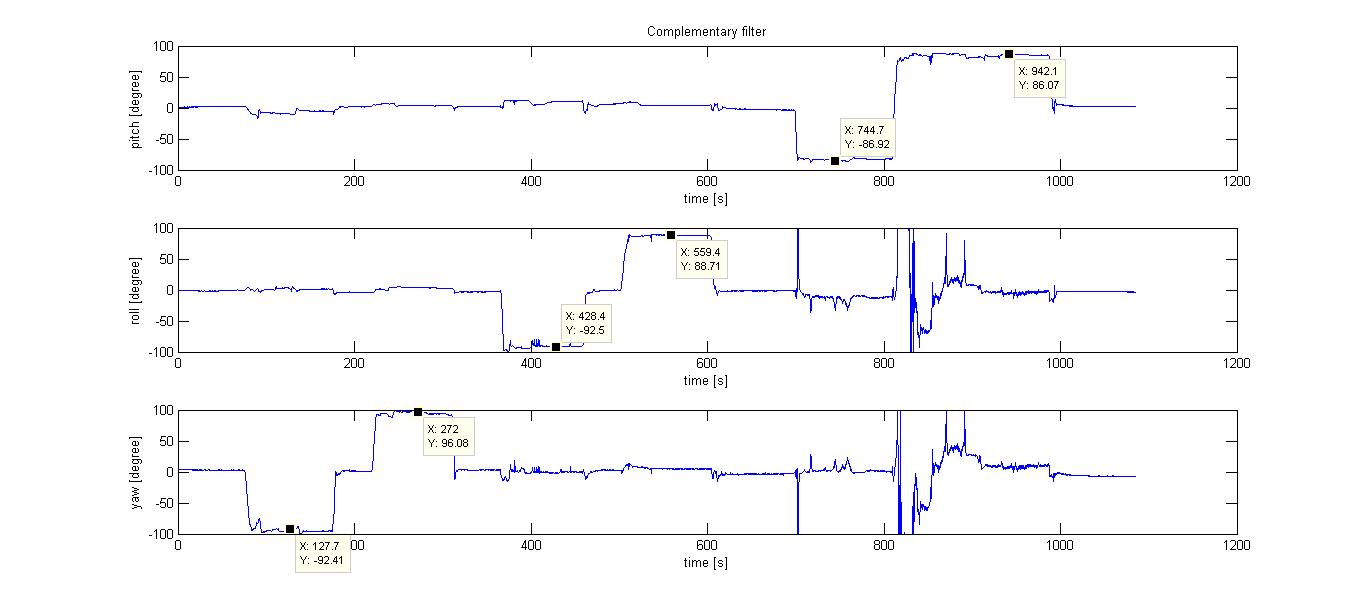
\includegraphics[width=1.0\textwidth]{fig/final_Comp1}
	\caption{Final result complementary filter}
	\label{fig:final_Comp}
\end{figure}
The comparison of the first result and the final result shows the increased filter speed. The signal needs not so much time to reach the final value. Also the yaw angle reaches the 90 degree when turning 90 degree. The extreme influences on yaw directly after changing of the rotation angle results from a hand made rotation. The influences on yaw while an other angle is applied is extremely reduced.\\

The last figure shows how off an angle can be when just an gyroscope is used. On the left side the integrated gyroscope can be seen. On the right side, the 3D representation of the fusioned sensors are displayed.
\begin{figure}[H]
	\centering\includegraphics[width=0.6\textwidth]{fig/3D}
	\caption{3D representation of the integrated gyroscope raw values on the left and the fusion filtered on the right}
	\label{fig:3D}
\end{figure}